
%(BEGIN_QUESTION)
% Copyright 2006, Tony R. Kuphaldt, released under the Creative Commons Attribution License (v 1.0)
% This means you may do almost anything with this work of mine, so long as you give me proper credit

Hvor stor lineær kraft vil bilens dekk utøve mot bakken dersom akselen påfører hjulet et dreiemoment på 1500 lb-ft, og dekkets radius er 11 tommer?

$$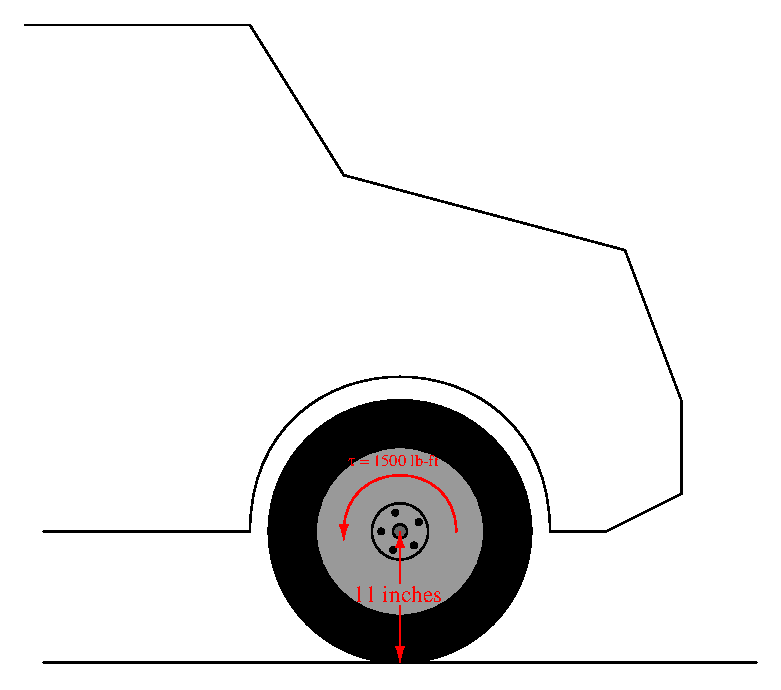
\includegraphics[width=15.5cm]{i01402x01.eps}$$

\underbar{file i01402}
%(END_QUESTION)





%(BEGIN_ANSWER)

$F$ = 1636.36 lb
 
\vskip 10pt

For å løse ut kraft trenger vi bare å omskrive momentligningen slik at kraft ($F$) står alene på én side av likhetstegnet:

$$\vec \tau = \vec r \times \vec F$$

$$\vec F = {\vec \tau \over \vec r}$$

Siden vi i denne oppgaven vet at alle tre vektorene er ortogonale (vinkelrette) på hverandre, kan vi skrive ligningen i enklere form med skalarstørrelser i stedet for vektorstørrelser:
 
$$F = {\tau \over r}$$

\vskip 10pt

Før vi kan sette inn oppgitte verdier for dreiemoment og momentarmens lengde, må vi konvertere lengdeenheten for momentarmen:

$$\hbox{(11 inches)(1 foot / 12 inches) = 0.916667 feet}$$

Nå kan vi løse for kraft:

$$F = {1500 \hbox{ lb-ft} \over 0.916667 \hbox{ ft}}$$

$$F = 1636.36 \hbox{ lb}$$
 
%(END_ANSWER)





%(BEGIN_NOTES)


%INDEX% Physics, torque: calculation problem

%(END_NOTES)

